\documentclass[tikz,border=8pt]{standalone}
% Shared look for every TikZ diagram. Load with \input{../../tools/tikz-style.tex}
\usepackage[T1]{fontenc}
\usepackage{lmodern}
\renewcommand{\sfdefault}{lmr}  % diagrams use the same serif as the text
\usetikzlibrary{arrows.meta, positioning, shapes.geometric, calc, fit, backgrounds}
\definecolor{cblue}{HTML}{4C78A8}
\definecolor{corange}{HTML}{F58518}
\definecolor{cgreen}{HTML}{54A24B}
\definecolor{cred}{HTML}{E45756}
\definecolor{cpurple}{HTML}{B279A2}
\definecolor{cgrey}{HTML}{6B6B6B}
\tikzset{
  every picture/.style={font=\sffamily, line width=1.2pt},
  box/.style={draw=#1, fill=#1!12, rounded corners=4pt, align=center, inner sep=7pt, minimum height=1.1cm},
  box/.default=cgrey,
  arrow/.style={-{Stealth[length=3mm]}, draw=cgrey, line width=1.4pt},
  title/.style={font=\sffamily\bfseries\Large},
  note/.style={font=\sffamily\small, text=cgrey, align=center},
}
\AtBeginDocument{\hyphenpenalty=10000 \exhyphenpenalty=10000}

\newcommand{\hcell}[4]{% x, y, text, colour
  \node[box=#4, minimum width=2.0cm, minimum height=0.8cm, inner sep=3pt, font=\sffamily\bfseries] at (#1,#2) {#3};}
\newcommand{\vcell}[4]{\node[draw=#4, fill=white, minimum width=2.0cm, minimum height=0.75cm] at (#1,#2) {#3};}
\begin{document}
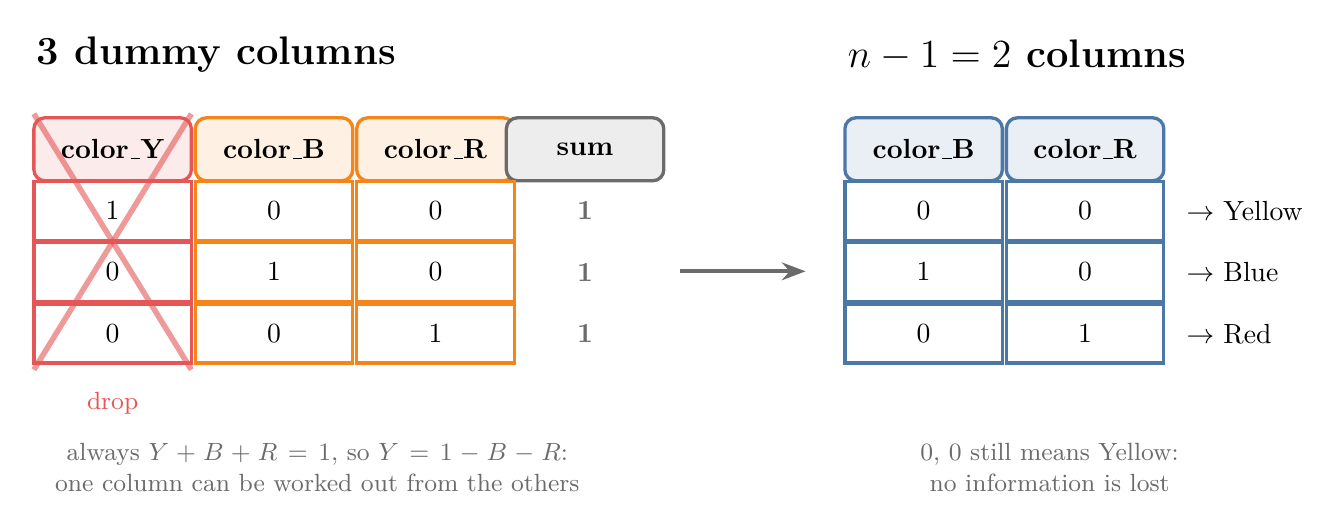
\begin{tikzpicture}
  % left: three dummy columns, row sums
  \node[title, anchor=west] at (-1.1,1.2) {3 dummy columns};
  \hcell{0}{0}{color\_Y}{cred}
  \hcell{2.05}{0}{color\_B}{corange}
  \hcell{4.1}{0}{color\_R}{corange}
  \hcell{6.0}{0}{sum}{cgrey}
  \foreach \a/\b/\c/\n [count=\i] in {1/0/0/Yellow, 0/1/0/Blue, 0/0/1/Red} {
    \vcell{0}{-0.78*\i}{\a}{cred}
    \vcell{2.05}{-0.78*\i}{\b}{corange}
    \vcell{4.1}{-0.78*\i}{\c}{corange}
    \node[font=\sffamily\bfseries, text=cgrey] at (6.0,-0.78*\i) {1};
  }
  \draw[cred, line width=2pt, opacity=0.6] (-1.0,0.45) -- (1.0,-2.8);
  \draw[cred, line width=2pt, opacity=0.6] (1.0,0.45) -- (-1.0,-2.8);
  \node[note, text=cred, anchor=north] at (0,-2.95) {drop};
  \node[note, anchor=north, text width=7cm] at (2.6,-3.6) {always $Y + B + R = 1$, so $Y = 1 - B - R$:\\ one column can be worked out from the others};
  \draw[arrow] (7.2,-1.55) -- (8.8,-1.55);
  % right: two columns, yellow is the baseline
  \begin{scope}[xshift=10.3cm]
  \node[title, anchor=west] at (-1.1,1.2) {$n-1 = 2$ columns};
  \hcell{0}{0}{color\_B}{cblue}
  \hcell{2.05}{0}{color\_R}{cblue}
  \foreach \b/\c/\n [count=\i] in {0/0/Yellow, 1/0/Blue, 0/1/Red} {
    \vcell{0}{-0.78*\i}{\b}{cblue}
    \vcell{2.05}{-0.78*\i}{\c}{cblue}
    \node[anchor=west, font=\sffamily] at (3.2,-0.78*\i) {$\rightarrow$ \n};
  }
  \node[note, anchor=north, text width=5.5cm] at (1.6,-3.6) {0, 0 still means Yellow:\\ no information is lost};
  \end{scope}
\end{tikzpicture}
\end{document}
